
\section{Sparsity-Aided Machine Unlearning}
\label{sec: sparsity_MU_alg}



%In the previous section, we showed that model sparsification could be a principled approach of reducing the gap between approximate unlearning and exact unlearning. 
Our study in Sec.\,\ref{sec: sparsityMU} suggests the new  {\MU} paradigm `prune first, then unlearn', which leverages the fact that  (approximate) unlearning on a sparse model yields a smaller unlearning error (Prop.\,\ref{prop: SGD_sparse_MU}) and improves the efficacy of {\MU}   (Fig.\,\ref{fig: results_OMP_MU}).
This promising finding, however, raises some new questions.  First, it remains elusive how the choice of a weight pruning method impacts the unlearning performance. Second,
%besides unlearning on a     sparse model,
it leaves room for developing  {sparsity-aware} {\MU} methods that can directly scrub data influence from a dense model.  %This section will address these two questions.
 



\noindent \textbf{Prune first, then unlearn: Choice of pruning methods.}
  % Our study in Sec.\,\ref{sec: sparsityMU} suggested the new  {\MU} paradigm `prune first, then unlearn', which shed light on that  (approximate) unlearning on a sparse model   yields a smaller unlearning error (Prop.\,\ref{prop: SGD_sparse_MU}) and improves the efficacy  of {\MU}   (Fig.\,\ref{fig: results_OMP_MU}).
  % Yet, 
  There exist many ways to find the desired sparse model
in addition to OMP. Examples include pruning at random
initialization before training \cite{tanaka2020pruning,frankle2020pruning}
 and simultaneous pruning-training iterative magnitude pruning (\textbf{IMP}) \cite{frankle2018lottery}.
  %Yet, there   exist many ways 
  %iterative magnitude pruning (\textbf{IMP}) \cite{ma2021sanity,frankle2018lottery}. 
  Thus, the problem of pruning method selection arises for {\MU}. From the viewpoint of {\MU},  the unlearner would prioritize a pruning method that satisfies the following criteria:  \ding{182} \textit{least dependence}  on the forgetting dataset ($\Df$), \ding{183} \textit{lossless generalization} when pruning, and \ding{184} \textit{pruning efficiency}. The rationale behind \ding{182} is  that  
  %since {\MU} targets scrubbing the influence of $\Df$ in the trained model, 
  it is desirable \textit{not} to incorporate    information of $\Df$ when seeking a sparse model prior to unlearning. 
  %\PS{This point is not clear to me. Additional info such as?} 
  And the criteria \ding{183} and \ding{184} ensure that sparsity cannot hamper {\TA} (testing accuracy)  and {\RTE} (run-time efficiency). 
  %which are also desired for {\MU} in addition to efficacy and fidelity (see Table\,\ref{tab: summary_MU_methods_metrics}).
  Based on \ding{182}-\ding{184}, 
  we   propose to use two pruning methods.  
  %in the `prune first, then unlearn' paradigm. 

\noindent  \ding{70} \textbf{SynFlow} (synaptic flow pruning) \cite{tanaka2020pruning}: 
SynFlow provides a (training-free) pruning method at initialization, even without   accessing the dataset. %to identify highly sparse sub-models  at initialization. 
Thus, it is uniquely suited for {\MU} to meet  the criterion \ding{182}. And SynFlow is easy to compute and yields a generalization improvement over many other pruning-at-initialization methods; see justifications in \cite{tanaka2020pruning}.


  
\noindent \ding{70} \textbf{OMP} (one-shot magnitude pruning)  \cite{ma2021sanity}: 
Different from SynFlow, {OMP}, which we focused on in Sec.\,\ref{sec: sparsityMU},
is performed over the original model   ($\thetafull$). It may depend on
%relate to \PS{``depend on''?}
%and thus  relates to 
the forgetting dataset ($\Df$), but has a much weaker dependence compared to {IMP}-based methods.
%Yet, such a relationship is much looser than     {IMP}-based methods \cite{frankle2018lottery}.
%that we have introduced and used in Sec.\,\ref{sec: sparsityMU} 
Moreover, {OMP} is  computationally lightest (\textit{i.e.}  best for \ding{184}) and    can yield better generalization than {SynFlow} \cite{zhang2022advancing}.
%Fig.\,\ref{fig: OMP_results} and Fig.\ref{fig: results_OMP_MU}


\begin{wrapfigure}{r}{72mm}
\vspace*{-4.5mm}
\centerline{
\begin{tabular}{cccc}
\hspace*{-5mm} 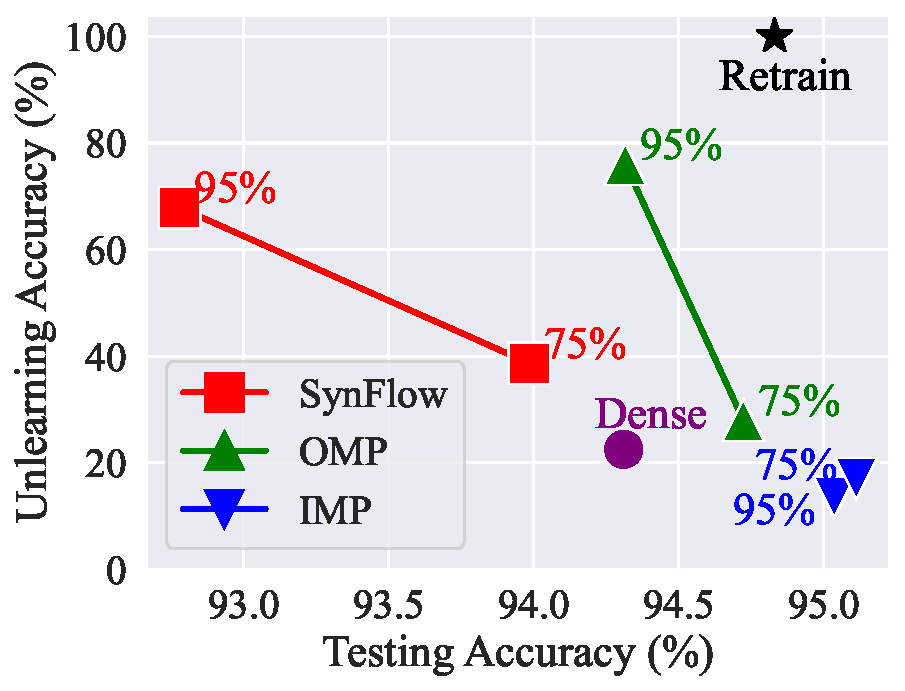
\includegraphics[width=35mm,height=!]{figs/UA_vs_pruning_retrain.pdf} &
    \hspace*{-5mm}  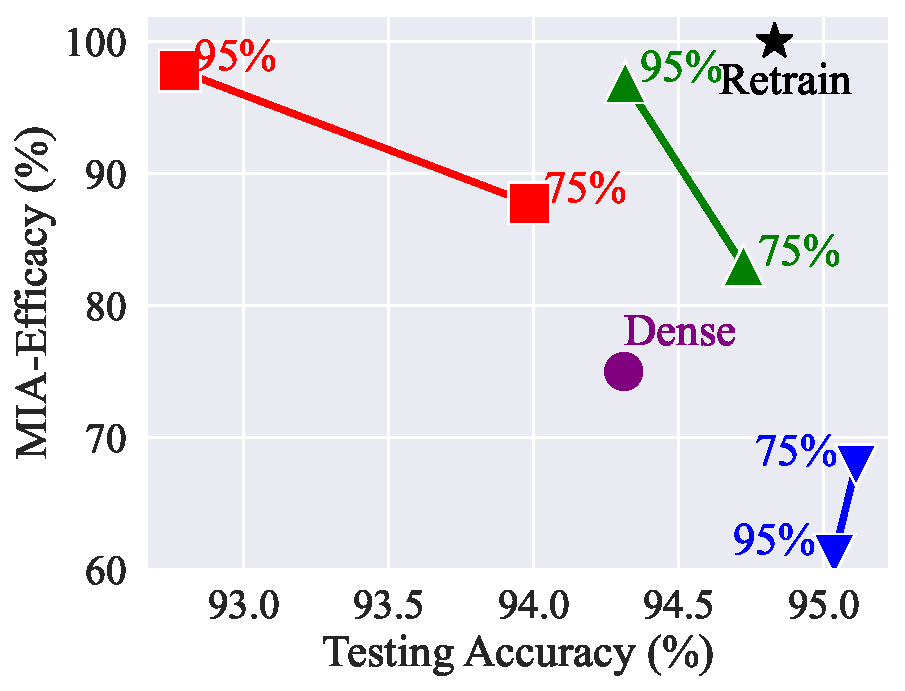
\includegraphics[width=35mm,height=!]{figs/MIA_vs_pruning.pdf} 
    \hspace*{-3mm} 
\end{tabular}}
 \vspace*{-3mm}
\caption{\footnotesize{Influence of different   pruning
methods ({\color{red}{SynFlow}}, {\color{ForestGreen}{OMP}}, and {\color{blue}{IMP}}) in unlearning efficacy ({\UA} and {\MIAF}) and generalization ({\TA})  on    (CIFAR-10, ResNet-18). \textbf{Left}: {\UA} vs. {\TA}. \textbf{Right}:   {\MIAF} vs. {\TA}. Each point is a {\FT}-based unlearned dense or sparse model (75\% or 95\% sparsity), or a retrained dense model.
%using  {\FT}. \JC{If a pruning method is proper for {\MU}, then its integration with {\FT} should  yield unlearned models with closer {\UA}, {\MIAF}, and {\TA} to {\retrain}.} 
%\JC{larger font in figs}
}}
 \vspace*{-4mm}
\label{fig: results_pruning_comparison}
\end{wrapfigure}
Furthermore, it is important to clarify that IMP (iterative magnitude pruning) is \textit{not} suitable for {\MU}, despite being widely used to find the most accurate sparse models (\textit{i.e.}, best for criterion \ding{183}).
% Next, we would like to highlight that IMP is not proper for {\MU} although it is the predominant approach to find the most accurate sparse models (\textit{i.e.},     best for \ding{183}). 
 % We also remark that in the research on model pruning, IMP   is   the predominant approach to find the most accurate sparse models (\textit{i.e.},     best for \ding{183}). 
 Compared with the proposed pruning methods, IMP has the largest computation overhead   and the strongest correlation with the training dataset (including $\Df$), thereby deviating from \ding{182} and \ding{184}.
 %due to its pruning-retraining iterations. 
 % In this sense, IMP may not be a proper  pruning choice for {\MU} through the lenses of \ding{182} and \ding{184}. 
 In \textbf{Fig.\,\ref{fig: results_pruning_comparison}}, we show  the   efficacy  of {\FT}-based unlearning on sparse models generated  using  different pruning methods (SynFlow, OMP, and IMP). 
 %where {\FF} is used as the unlearning algorithm.
 %the unlearning setup remains the same as Fig.\,\ref{fig: results_OMP_MU}.  
 As we can see, unlearning on {SynFlow} or {OMP}-generated sparse models yields improved {\UA} and {\MIAF} over that on the original dense model and   {IMP}-generated sparse models.  This unlearning improvement over the dense model is consistent with Fig.\,\ref{fig: results_OMP_MU}. More interestingly, we find that {IMP} \textit{cannot} benefit the unlearning efficacy, although it leads to the best {\TA}. This is because {IMP} heavily relies on the training set including forgetting data points, which is revealed by the empirical results -- the unlearning metrics get worse for IMP with increasing sparsity.
 %\textit{i.e.}, violating the criterion \ding{182}. 
 %We will  show a fix to {IMP} for {\MU} later.
 Furthermore, when examining the performance of SynFlow and OMP, we observe that the latter   generally outperforms the former, exhibiting results that are closer to those of {\retrain}. 
 %in {\TA} with  similar unlearning efficacy.  
 Thus,  \textit{{OMP} is the pruning method we will use by default}. 
 
 
 %at the model sparsity ratios 75\% and 95\%
 
 %compared to SynFlow and IMP, 
 
 %\SL{[add experiment analysis and distilled unlearning principles/insights. @Jiancheng, @Jinghan]}



%% While IMP is powerful, it requires multiple cycles of
%expensive training and pruning with very specific sets of hyperparameters.


%%% empirical results



%To this end, we  propose two sparsity-aware (approximate) unlearning methods below.

%built upon sparsity-regularized optimization   and pruning-unlearning alternative optimization (AO), respectively.  

%
\begin{wrapfigure}{r}{35mm}
\vspace*{-3mm}
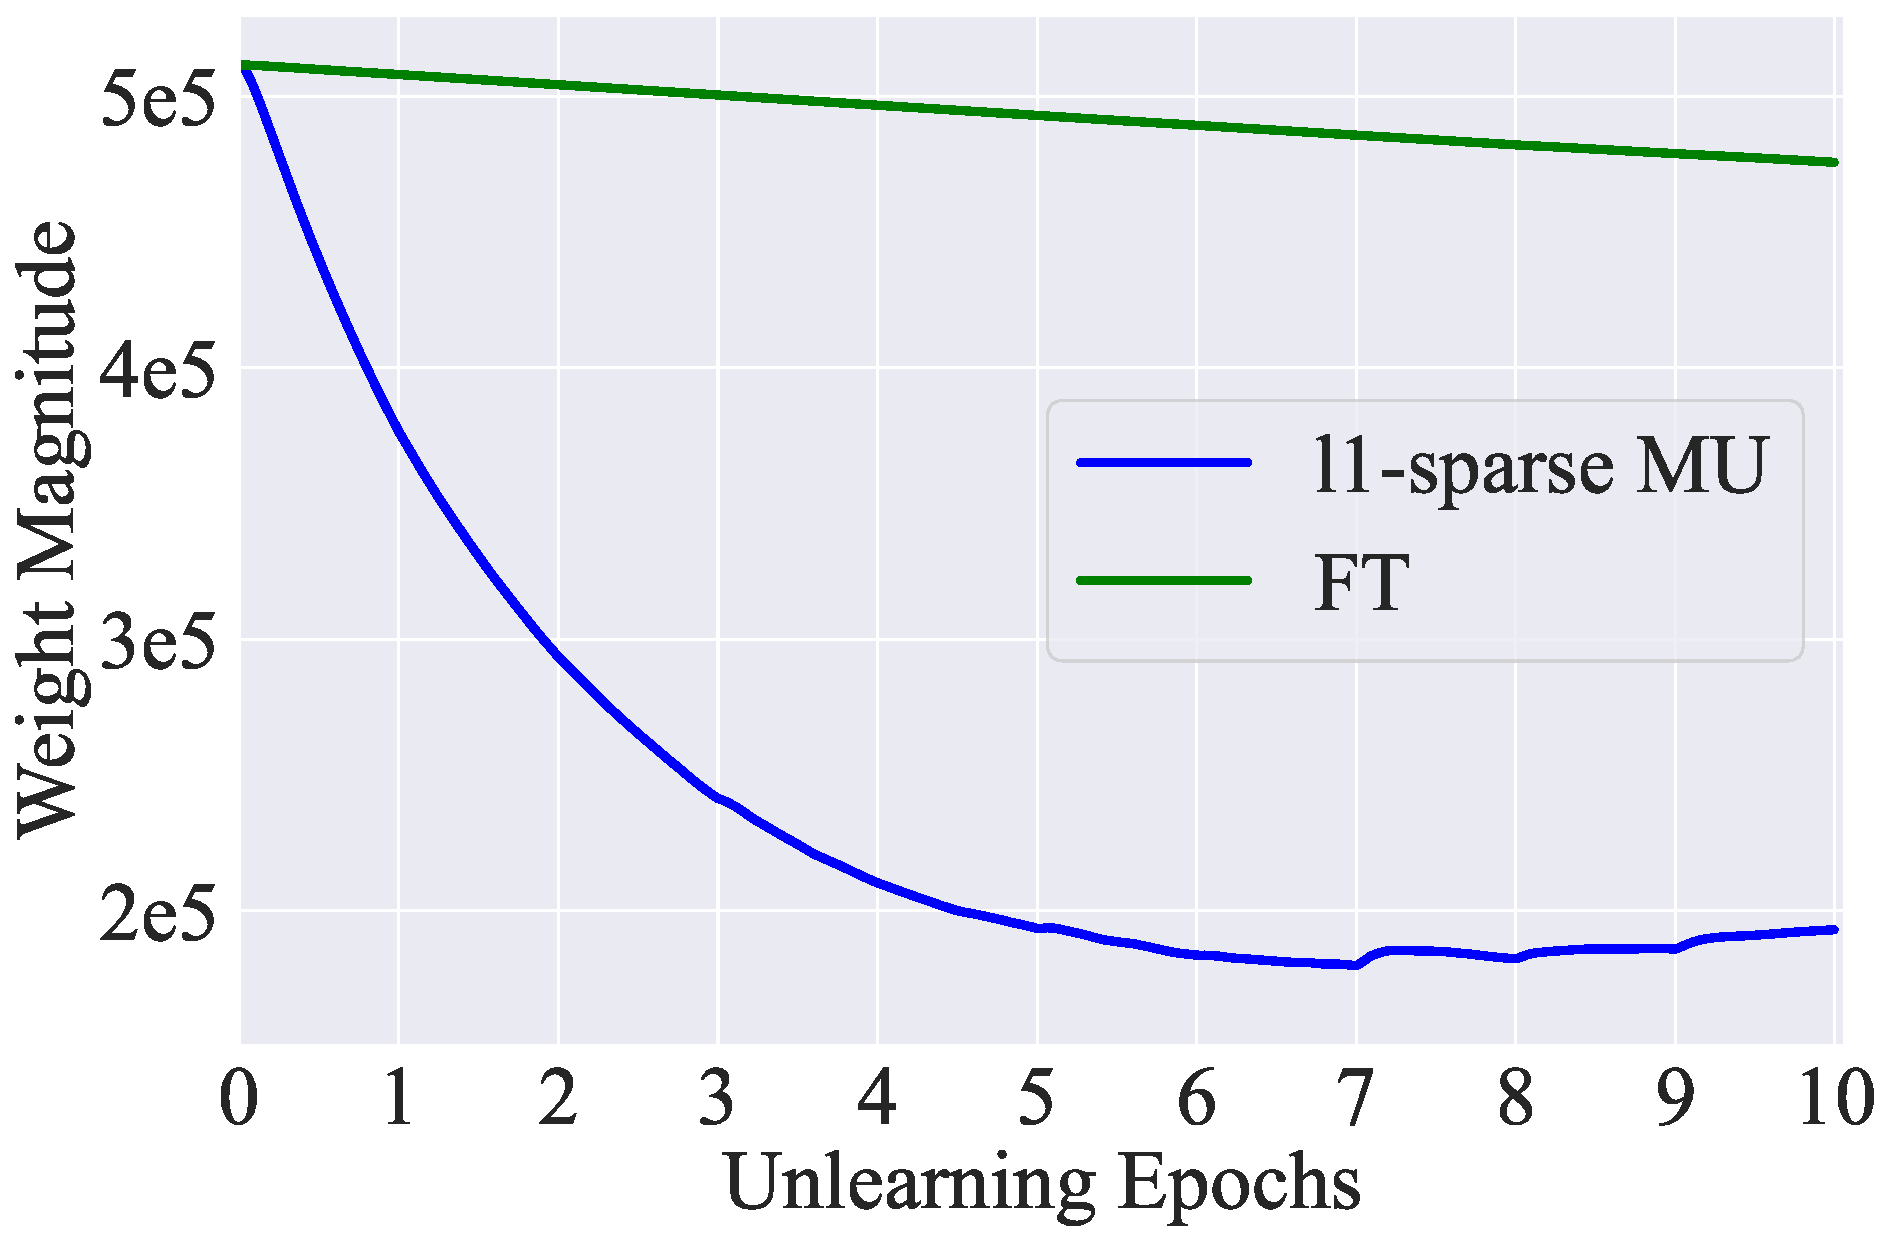
\includegraphics[width=35mm,height=!]{figs/magnitude.pdf}
\caption{\JC{Magnitude trend of the model weights during unlearning.}
\SL{Move to an appendix or delete.}}
\label{fig: l1_weight_magnitude}
\vspace*{-3mm}
\end{wrapfigure}
{\noindent \textbf{Sparsity-aware  unlearning.}}
% \JH{Add discussion about schedulers of $\gamma$, refer to table\,\ref{tab: ablation_l1_scheduler}.Also add some figures to show changes of magnitude.}
%In the   `prune first, then unlearn' paradigm, model sparsity is given \textit{a priori} for {\MU}. 
We next study if pruning and unlearning can be carried out simultaneously, without requiring prior knowledge of model sparsity. Let $\Lunl (\btheta; \thetafull,  \Dr)$ denote the unlearning objective function of model parameters $\btheta$, given the pre-trained  state $\thetafull$, 
%the overall training dataset $\mathcal D$, 
and the remaining training dataset $\Dr$. %Recall that $\Lunl $ can be specified by any {\MU} method studied in Sec.\,\ref{sec: primer_MU}. 
Inspired by  sparsity-inducing optimization \cite{bach2012optimization}, we integrate an $\ell_1$ norm-based sparse penalty into  $\Lunl $. This leads to the problem of `\textbf{\MUSparse}':

\vspace*{-3mm}
{\small{\begin{align}
    \thetaunl = \argmin_{\btheta} \Lunl (\btheta; \thetafull,  \Dr) + \gamma \| \btheta \|_1,
    \label{eq: MUSparse}
\end{align}}}%
where we specify $\Lunl$ by the fine-tuning objective, and $\gamma > 0$ is a regularization parameter that {controls the penalty level of the $\ell_1$ norm, thereby reducing the magnitudes of `unimportant' weights.}

%\noindent \textbf{\JC{Ablation study on parameter scheduler in \MUSparse.}}
% However, as \citep{bach2012optimization} mentioned, the downside of $\ell_1$ regulation term will affect the is its loss  in {\RA} and {\TA} compared to {\FT} and {\retrain}. Therefore, we conducted a comprehensive study of the scheduler of $\lambda$ in {\MUSparse}. In \textbf{Tab.\,\ref{tab: ablation_l1_scheduler}}, we present the results of unlearning performance on different parameter schedulers: constant scheduler, linear growing scheduler, and linear decaying scheduler.
% It shows that the decaying $\gamma$ scheduler performs the best among all the schedulers. If we directly apply a constant $\lambda$ to {\MUSparse}, it will either get a low {\UA} with lower $\lambda$ (for $\lambda = 0$, the method reduces to {\FT}) or worse {\RA} and {\TA} 
%  under higher $\lambda$. In Tab.\,\ref{tab: ablation_l1_scheduler}, we picked a sweet point to get a balance between them. If we use the linear growing scheduler, which means the method focuses on the unlearning term first then moves the focus to sparsity. If we use the linear decaying scheduler, the method focuses on the unlearning term first then moves the focus to sparsity.
\iffalse
\begin{wraptable}{R}{80mm}
\centering
\vspace*{-4.25mm}
\caption{\footnotesize{{\MU} performance  comparison of using {\MUSparse} with different   sparsity schedulers of $\gamma$  in \eqref{eq: MUSparse} and using {\retrain}.  
The unlearning scenario is given by random data forgetting (10\% data points across all classes) on (ResNet-18, CIFAR-10).
%considering various unlearning scenarios on CIFAR10 dataset. The content format follows Tab.\,\ref{tab: overall_perfoamnce}.
%Bold numbers indicate the closest performance to {\retrain}, and
A performance gap  against \textcolor{blue}{{\retrain}} is provided 
%. The relative drop or improvement represented 
in (\textcolor{blue}{$\bullet$}).
}}
\label{tab: ablation_l1_scheduler}
% \vspace*{0.1in} % Requirements, do not delete.
\resizebox{0.57\textwidth}{!}{
\begin{tabular}{c|c|c|c|c|c}
\toprule[1pt]
\midrule
  {\MU}& {\UA} & {{\MIAF}}& {{\RA}} & {{\TA}} & {{RTE} (min)} \\ 

% \cline{3-10}

% \midrule
% \rowcolor{Gray}
% \multicolumn{6}{c}{Class-wise forgetting} \\
% \midrule
% {\retrain} & \textcolor{blue}{100.00} & \textcolor{blue}{100.00} & \textcolor{blue}{100.00} & \textcolor{blue}{94.83} & 43.23
% \\
% {\MUSparse} + constant $\gamma$ & 100.00 (\textcolor{blue}{0.00}) & 100.00 (\textcolor{blue}{0.00}) & 91.69 (\textcolor{blue}{8.31})	& 87.3 (\textcolor{blue}{7.53}) & 2.61
% \\
% {\MUSparse} +   growing $\gamma$  & 100.00 (\textcolor{blue}{0.00}) & 100.00 (\textcolor{blue}{0.00}) & 94.43 (\textcolor{blue}{5.57})	& 88.43 (\textcolor{blue}{6.40}) & 2.61
% \\
% {\MUSparse} +   decaying $\gamma$ & 100.00 (\textcolor{blue}{0.00}) & 100.00 (\textcolor{blue}{0.00}) & \textbf{98.99} (\textcolor{blue}{\textbf{1.01}})	& \textbf{93.40} (\textcolor{blue}{\textbf{1.43}}) & 2.61
% \\
% \midrule
% \rowcolor{Gray}
% \multicolumn{6}{c}{Random data forgetting (all classes)} \\
\midrule
{\retrain} & \textcolor{blue}{5.41} & \textcolor{blue}{13.12} & \textcolor{blue}{100.00} & \textcolor{blue}{94.42} & 42.15
\\
%  \FT & $6.83$ (\textcolor{blue}{$1.42$}) & $14.97$ (\textcolor{blue}{$1.85$})& $96.61$ (\textcolor{blue}{$3.39$})& $90.13$ (\textcolor{blue}{$4.29$})  & 2.33 
% \\		
% \IU & $2.03$ (\textcolor{blue}{$3.38$})&  $5.07$ (\textcolor{blue}{$8.05$})& $98.26$ (\textcolor{blue}{$1.74$})& $\textbf{91.33}$ (\textcolor{blue}{$\textbf{3.09}$}) & 3.22
% \\
{\MUSparse} + constant $\gamma$ & 6.60 (\textcolor{blue}{1.19}) & 14.64 (\textcolor{blue}{1.52}) & 96.51 (\textcolor{blue}{3.49})	& 87.30 (\textcolor{blue}{7.53}) & 2.53
\\

{\MUSparse} + linear growing $\gamma$  & 3.80 (\textcolor{blue}{1.61}) & 8.75 (\textcolor{blue}{4.37}) & 97.13 (\textcolor{blue}{2.87})	& 90.63 (\textcolor{blue}{3.79}) & 2.53
\\
{\MUSparse} + linear decaying $\gamma$ & \textbf{5.35} (\textcolor{blue}{\textbf{0.06}}) & \textbf{12.71} (\textcolor{blue}{\textbf{0.41}}) & \textbf{97.39} (\textcolor{blue}{\textbf{2.61}})	& {\textbf{91.26}} (\textcolor{blue}{\textbf{3.16}}) & 2.53
\\
\midrule
\bottomrule[1pt]
\end{tabular}
}
\vspace*{-4mm}
\end{wraptable}
\fi
\vspace{-5mm}
\begin{table}[htb!]
\centering
\caption{\footnotesize{{\MU} performance  comparison of using {\MUSparse} with different   sparsity schedulers of $\gamma$  in \eqref{eq: MUSparse} and using {\retrain}.  
The unlearning scenario is given by random data forgetting (10\% data points across all classes) on (ResNet-18, CIFAR-10).
%considering various unlearning scenarios on CIFAR10 dataset. The content format follows Tab.\,\ref{tab: overall_perfoamnce}.
%Bold numbers indicate the closest performance to {\retrain}, and
A performance gap  against \textcolor{blue}{{\retrain}} is provided 
%. The relative drop or improvement represented 
in (\textcolor{blue}{$\bullet$}).
}}
\label{tab: ablation_l1_scheduler}
\vspace*{1mm}
% \vspace*{0.1in} % Requirements, do not delete.
\resizebox{0.85\textwidth}{!}{
\begin{tabular}{c|c|c|c|c|c}
\toprule[1pt]
\midrule
  {\MU}& {\UA} & {{\MIAF}}& {{\RA}} & {{\TA}} & {{RTE} (min)} \\ 

% \cline{3-10}

% \midrule
% \rowcolor{Gray}
% \multicolumn{6}{c}{Class-wise forgetting} \\
% \midrule
% {\retrain} & \textcolor{blue}{100.00} & \textcolor{blue}{100.00} & \textcolor{blue}{100.00} & \textcolor{blue}{94.83} & 43.23
% \\
% {\MUSparse} + constant $\gamma$ & 100.00 (\textcolor{blue}{0.00}) & 100.00 (\textcolor{blue}{0.00}) & 91.69 (\textcolor{blue}{8.31})	& 87.3 (\textcolor{blue}{7.53}) & 2.61
% \\
% {\MUSparse} +   growing $\gamma$  & 100.00 (\textcolor{blue}{0.00}) & 100.00 (\textcolor{blue}{0.00}) & 94.43 (\textcolor{blue}{5.57})	& 88.43 (\textcolor{blue}{6.40}) & 2.61
% \\
% {\MUSparse} +   decaying $\gamma$ & 100.00 (\textcolor{blue}{0.00}) & 100.00 (\textcolor{blue}{0.00}) & \textbf{98.99} (\textcolor{blue}{\textbf{1.01}})	& \textbf{93.40} (\textcolor{blue}{\textbf{1.43}}) & 2.61
% \\
% \midrule
% \rowcolor{Gray}
% \multicolumn{6}{c}{Random data forgetting (all classes)} \\
\midrule
{\retrain} & \textcolor{blue}{5.41} & \textcolor{blue}{13.12} & \textcolor{blue}{100.00} & \textcolor{blue}{94.42} & 42.15
\\
%  \FT & $6.83$ (\textcolor{blue}{$1.42$}) & $14.97$ (\textcolor{blue}{$1.85$})& $96.61$ (\textcolor{blue}{$3.39$})& $90.13$ (\textcolor{blue}{$4.29$})  & 2.33 
% \\		
% \IU & $2.03$ (\textcolor{blue}{$3.38$})&  $5.07$ (\textcolor{blue}{$8.05$})& $98.26$ (\textcolor{blue}{$1.74$})& $\textbf{91.33}$ (\textcolor{blue}{$\textbf{3.09}$}) & 3.22
% \\
{\MUSparse} + constant $\gamma$ & 6.60 (\textcolor{blue}{1.19}) & 14.64 (\textcolor{blue}{1.52}) & 96.51 (\textcolor{blue}{3.49})	& 87.30 (\textcolor{blue}{7.12}) & 2.53
\\

{\MUSparse} + linear growing $\gamma$  & 3.80 (\textcolor{blue}{1.61}) & 8.75 (\textcolor{blue}{4.37}) & 97.13 (\textcolor{blue}{2.87})	& 90.63 (\textcolor{blue}{3.79}) & 2.53
\\
{\MUSparse} + linear decaying $\gamma$ & \textbf{5.35} (\textcolor{blue}{\textbf{0.06}}) & \textbf{12.71} (\textcolor{blue}{\textbf{0.41}}) & \textbf{97.39} (\textcolor{blue}{\textbf{2.61}})	& {\textbf{91.26}} (\textcolor{blue}{\textbf{3.16}}) & 2.53
\\
\midrule
\bottomrule[1pt]
\end{tabular}
}
\end{table}
In practice,  the unlearning performance could be sensitive to the choice of the sparse regularization parameter $\gamma$. To address this limitation, we propose the design of a sparse regularization scheduler. Specifically, we explore three schemes: (1) constant $\gamma$, (2) linearly growing $\gamma$ and (3) linearly decaying $\gamma$; see Sec.\,\ref{sec: exp_setup} for detailed implementations. Our empirical evaluation presented in \textbf{Tab.\,\ref{tab: ablation_l1_scheduler}} shows that the use of a linearly decreasing $\gamma$ scheduler outperforms   other schemes.  
This scheduler not only minimizes the gap in unlearning efficacy compared to {\retrain}, but also improves the preservation of {\RA} and {\TA} after unlearning. 
These findings suggest that it is advantageous to prioritize promoting sparsity during the early stages of unlearning and then gradually shift the focus towards enhancing fine-tuning accuracy on the remaining dataset $\Dr$.

% As Sec.\,\ref{sec: sparsity_MU_alg} pointed out, the downside of the $\ell_1$ regularization term is its suppression on {\RA} and {\TA} compared to {\FT} and {\retrain}. To facilitate this deficiency, we introduced a well-designed scheduler to $\gamma$, the parameter of the regularization term, and conducted a comprehensive ablation study on designing the scheduler. The results of unlearning performance with different parameter schedulers, constant, linearly increasing, and linearly decreasing schedulers, are presented in \textbf{Tab.\,\ref{tab: ablation_l1_scheduler}}.

% Directly applying a constant $\gamma$ to {\MUSparse} would either yield a low unlearning efficacy with lower $\gamma$ (for $\gamma = 0$, the method reduces to {\FT}) or degraded generalization performance under higher $\gamma$. In \textbf{Tab.\,\ref{tab: ablation_l1_scheduler}}, we have identified an optimal point that balances these metrics. Still, it cannot achieve as good performance as scheduled $\gamma$. The linearly increasing scheduler implies that the method initially emphasizes the unlearning term, then gradually shifts its focus towards sparsity. Conversely, the linearly decaying scheduler suggests that the focus initially lands on the sparsity, then gradually shifts to the unlearning term. The results reveal that the decaying scheduler outperforms all the others on both class-wise forgetting and random data forgetting, which aligned with the inspiration of the `prune first, then unlearn' paradigm. Therefore, the decaying scheduler will use in successive experiments except specified otherwise.

%controls the sparsity of the model parameters in $\btheta$.  
%In \eqref{eq: MUSparse},   \SL{we specify $\Lunl$ by the fine-tuning objective}.  
%leading to the {\FT}-oriented {\MUSparse}. 
% \JC{\textbf{Fig.}\,\ref{fig: l1_weight_magnitude} shows during the {\MUSparse}, the variation tendency of the magnitude among the epochs, compared with {\FT}.}
% \JC{Moreover, since the $\ell_1$ regularizer would dampen the model's generalization performance, in order to get a balance between the impact of two terms, we used a decaying parameter schedule to $\gamma$. For further analysis and ablation studies on the scheduler selection, please refer to Sec.\,\ref{sec: experiment_results}.}

%\JC{\textbf{Fig.}\,\ref{fig: l1_weight_magnitude} illustrates the variation in magnitude among the epochs during the {\MUSparse} process, in comparison with {\FT}.}





% \JC{Furthermore, as the $\ell_1$ regularizer may dampen the model's generalization performance, we employ a decaying parameter schedule for $\gamma$ to gain advantages from both of the two terms. For a more in-depth analysis and ablation studies on scheduler selection, please refer to Sec.\,\ref{sec: experiment_results}.}

% \JC{ablation study on scheduler}

 
 %\SL{[Mention what existing unlearning objectives to be integrated with above proposal?]}
% \JC{remove AO?}
% In addition to \eqref{eq: MUSparse}, we can integrate pruning with unlearning via alternating optimization (\textbf{AO}) taking inspiration from the IMP algorithm \cite{frankle2018lottery}. Yet, different from IMP,  we replace the optimization step of retraining non-zero weights with unlearning on non-zero model weights. We term the resulting  method `\textbf{\MUAO}' and summarize its pipeline (S1)-(S3) below. 
% \textbf{(S1)} \textit{Initialize} model     $\btheta = \thetafull$ and a  pruning   mask $\mathbf m = \mathbf 1$.
% \textbf{(S2)}   \textit{Prune} $p\%$ non-zero parameters in $\btheta$ per magnitude. Then, update $\mathbf m$ to a sparser mask.
% \textbf{(S3)}  \textit{Unlearn} $\Df$ on the sparse model $\mathbf m \odot \btheta$ using an approximate unlearning method (\textit{e.g.}, {\FT}) to update the non-zero model parameters and go back to (S2).
% The above procedure \textbf{(S1)}$\to$\textbf{(S2)}$\rightleftarrows$\textbf{(S3)}  
%  repeatedly prunes and unlearns the model over multiple rounds (assuming $k$ rounds). Similar to IMP in \cite{frankle2018lottery},  we adopt a progressive learning process, where  each round prunes $p^{1/k}$\% of the weights on top of the previous round ($p=20\%$ by default). However, different from IMP,  {\MUAO} is much lighter in computation since approximate unlearning in (S2) takes fewer computation overheads than   retraining non-zero model weights in IMP.  


\iffalse 
We integrate two efficient unlearning methods {\FT} and {\GA} with these two proposed sparse-aware unlearning methods. In what follows, we will only report the {\FT}, which outperforms {\GA} integrated with sparsity-aware methods (shown in Table\,\ref{} \JH{appendix}).    
 \SL{[Mention what existing unlearning objectives to be integrated with above proposal?]}
 \fi 